\documentclass{article}
\usepackage{tikz}
\usetikzlibrary{arrows,backgrounds,calc,trees}

\pgfdeclarelayer{background}
\pgfsetlayers{background,main}


\newcommand{\convexpath}[2]{
[   
    create hullnodes/.code={
        \global\edef\namelist{#1}
        \foreach [count=\counter] \nodename in \namelist {
            \global\edef\numberofnodes{\counter}
            \node at (\nodename) [draw=none,name=hullnode\counter] {};
        }
        \node at (hullnode\numberofnodes) [name=hullnode0,draw=none] {};
        \pgfmathtruncatemacro\lastnumber{\numberofnodes+1}
        \node at (hullnode1) [name=hullnode\lastnumber,draw=none] {};
    },
    create hullnodes
]
($(hullnode1)!#2!-90:(hullnode0)$)
\foreach [
    evaluate=\currentnode as \previousnode using \currentnode-1,
    evaluate=\currentnode as \nextnode using \currentnode+1
    ] \currentnode in {1,...,\numberofnodes} {
-- ($(hullnode\currentnode)!#2!-90:(hullnode\previousnode)$)
  let \p1 = ($(hullnode\currentnode)!#2!-90:(hullnode\previousnode) - (hullnode\currentnode)$),
    \n1 = {atan2(\x1,\y1)},
    \p2 = ($(hullnode\currentnode)!#2!90:(hullnode\nextnode) - (hullnode\currentnode)$),
    \n2 = {atan2(\x2,\y2)},
    \n{delta} = {-Mod(\n1-\n2,360)}
  in 
    {arc [start angle=\n1, delta angle=\n{delta}, radius=#2]}
}
-- cycle
}

\begin{document}
\thispagestyle{empty}

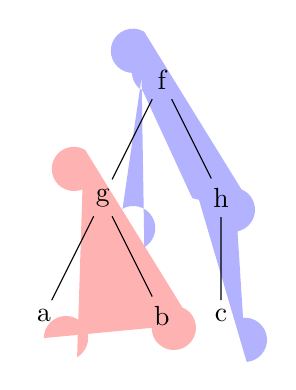
\begin{tikzpicture}
\node (f) {f}
    child { node (g) {g} 
      child { node (a) {a}
    }
      child { node (b) {b}
    }
  }
    child { node (h) {h}
      child { node (c) {c}
    }
  };
\begin{pgfonlayer}{background}
\fill[red,opacity=0.3] \convexpath{a,g,b}{8pt};
\fill[blue,opacity=0.3] \convexpath{g,f,h,c,h,f}{8pt};
\end{pgfonlayer}
\end{tikzpicture}

\end{document}